\section{Modèles d'architecture}

\paragraph{} Le réseau de téléphonie de l'INSA actuel couvre actuellement le
support de 3000 postes téléphoniques. Le déploiement du réseau de téléphonie par
IP sur le campus de l'INSA ne peut être réalisé en rupture avec cette
infrastructure analogique existante.

\paragraph{} La section qui suit décrira à un niveau conceptuel l'architecture
du réseau de téléphonie existant, de celui que nous proposons à terme, et de
celui que nous proposons durant la phase de transition.

\subsection{Architecture existante}
\paragraph{} L'architecture actuelle repose sur un PABX analogique chargé
d'effectuer la commutation des lignes et d'assurer la liaison vers le réseau
\ac{RNIS} de l'opérateur. Cette architecture est présentée graphiquement dans la
figure \ref{synoptique_existant}.

\begin{figure}[h]
  \caption{\label{synoptique_existant} Synoptique du réseau de téléphonie
    existant}
  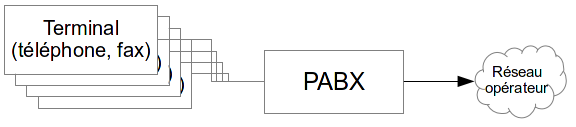
\includegraphics{Existant.png}
\end{figure}

\subsection{Architecture de transition}
\paragraph{} L'objectif de l'architecture de transition est d'intégrer
le réseau ToIP au réseau existant, pour progressivement pouvoir basculer des
postes du réseau analogique vers le réseau numérique. Cette architecture est
présentée graphiquement dans la figure \ref{synoptique_transition}.

\begin{figure}[h]
  \caption{\label{synoptique_transition} Synoptique du réseau de téléphonie de
    transition}
  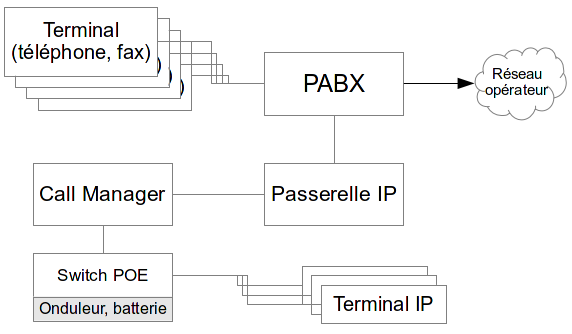
\includegraphics{Transition.png}
\end{figure}

\paragraph{} Le réseau IP va être progressivement déployé sur sa "propre
branche" du réseau de téléphonie. Il sera intégré au réseau analogique existant
(qui dans un premier temps doit être intégralement conservé) grâce à une
passerelle IP.

\paragraph{} La passerelle IP est un dispositif offrant ensemble d'interfaces
réseau qui permettent de relier un réseau de téléphonie IP et un réseau
téléphonique analogique. Le choix du matériel sera discuté plus tard.

\paragraph{} Le Call Manager est un serveur disposant d'un ensemble de logiciels
permettant d'administrer le réseau de ToIP. La fonction principale du Call
Manager est d'attribuer une ligne (un numéro) à un poste téléphonique ou une IP.
Selon les capacités des logiciels utilisés, le Call Manager peut permettre
d'appliquer des règles de gestions complémentaires (quotas, filtrages,
redirection d'appels, etc).

\paragraph{} Le réseau sera déployé avec des switchs POE (Power Over Ethernet),
afin de garantir le bon fonctionnement des téléphones en cas de pannes,
notamment électrique. Le cæur du réseau est lui sécurisé grâce au moyens
mis en place pour sécuriser le réseau du campus (groupe électrogène). Les
téléphones IP seront reliés à ces switchs.

\paragraph{} Nous souhaitons utiliser tant que possible le réseau Ethernet
existant. Nous utiliserons donc des téléphones offrant deux interfaces RJ45 et
qui permettent de connecter un ordinateur en "bout de ligne".

\subsection{Architecture cible}
\paragraph{} L'architecture cible se passera du PABX actuel, qui arrivera en fin
de vie. Les terminaux analogiques "résiduels" seront reliés à la passerelle IP à
l'aide d'interfaces RJ11 spécifiques.

\paragraph{} La liaison avec le réseau opérateur se fera au niveau du serveur
Call Manager, qui sera équipé des interfaces réseau adéquates. Il ne jouera plus
simplement le rôle de Call Manager, mais peut être vu comme un IPBX complet.
La variation sémantique implique ici la liaison directe avec le réseau
opérateur. Cette architecture est présentée graphiquement dans la figure
\ref{synoptique_cible}.

\begin{figure}[h]
  \caption{\label{synoptique_cible} Synoptique du réseau de téléphonie cible}
  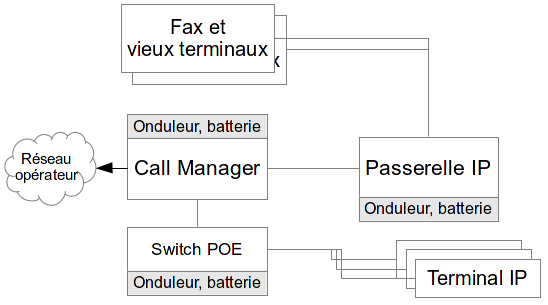
\includegraphics{Cible.png}
\end{figure}
